
\begin{figure}[H]
  {
    \setlength{\tabcolsep}{3.0pt}
    \setlength\cmidrulewidth{\heavyrulewidth} % Make cmidrule = 
    \begin{adjustbox}{height=5cm,center}
      \footnotesize
      \begin{tabular}{ll}

        \makecell[l]{
\icode{.BYTE \$01,\$01,\$FF,\$FF}\\
\icode{.BYTE \$FF,\$01,\$01,\$FF}
} & \makecell[l]{

\includegraphics[width=1.3cm]{src/patterns/pixels/pixel_pattern6_0.png}%
} \\
        \midrule

        \makecell[l]{
\icode{.BYTE \$02,\$02,\$FE,\$FE}\\
\icode{.BYTE \$FE,\$02,\$02,\$FE}
} & \makecell[l]{

\includegraphics[width=1.3cm]{src/patterns/pixels/pixel_pattern6_1.png}%

\includegraphics[width=1.3cm]{src/patterns/pixels/pixel_pattern6_2.png}%
} \\
        \midrule

        \makecell[l]{
\icode{.BYTE \$01,\$03,\$03,\$01,\$FF,\$FD,\$FD,\$FF}\\
\icode{.BYTE \$FD,\$FF,\$01,\$03,\$03,\$01,\$FF,\$FD}
} & \makecell[l]{

\includegraphics[width=1.3cm]{src/patterns/pixels/pixel_pattern6_3.png}%

\includegraphics[width=1.3cm]{src/patterns/pixels/pixel_pattern6_4.png}%

\includegraphics[width=1.3cm]{src/patterns/pixels/pixel_pattern6_5.png}%
} \\
        \midrule

        \makecell[l]{
\icode{.BYTE \$03,\$03,\$FD,\$FD}\\
\icode{.BYTE \$FD,\$03,\$03,\$FD}
} & \makecell[l]{
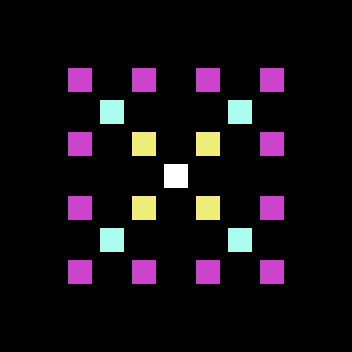
\includegraphics[width=1.3cm]{src/patterns/pixels/pixel_pattern6_6.png}%
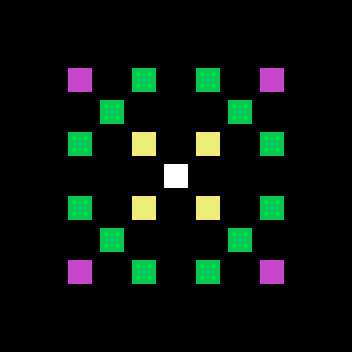
\includegraphics[width=1.3cm]{src/patterns/pixels/pixel_pattern6_7.png}%
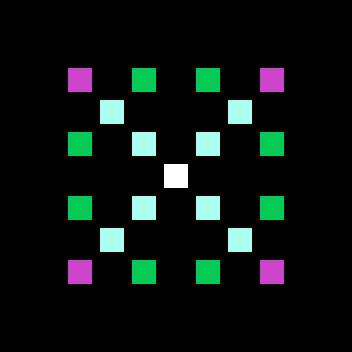
\includegraphics[width=1.3cm]{src/patterns/pixels/pixel_pattern6_8.png}%
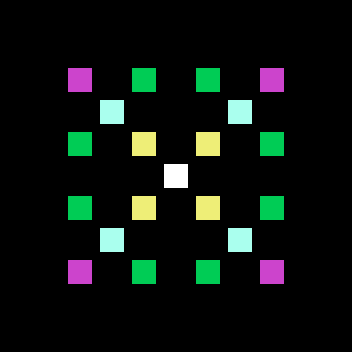
\includegraphics[width=1.3cm]{src/patterns/pixels/pixel_pattern6_9.png}%
} \\
        \midrule

        \makecell[l]{
\icode{.BYTE \$04,\$04,\$FC,\$FC}\\
\icode{.BYTE \$FC,\$04,\$04,\$FC}
} & \makecell[l]{
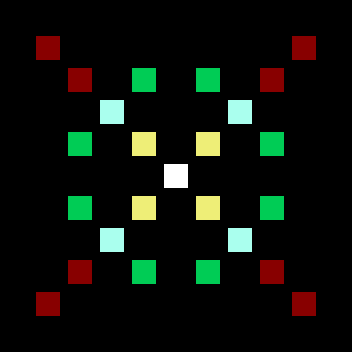
\includegraphics[width=1.3cm]{src/patterns/pixels/pixel_pattern6_10.png}%
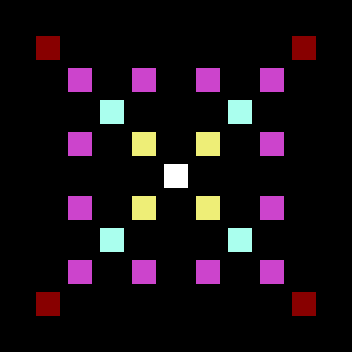
\includegraphics[width=1.3cm]{src/patterns/pixels/pixel_pattern6_11.png}%
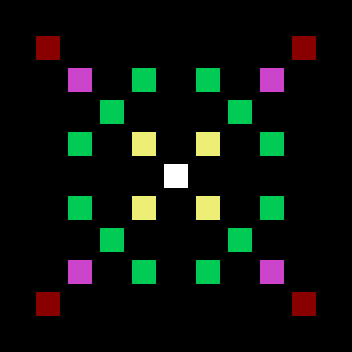
\includegraphics[width=1.3cm]{src/patterns/pixels/pixel_pattern6_12.png}%
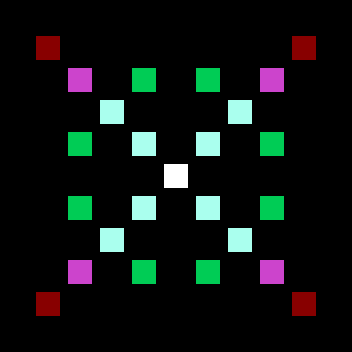
\includegraphics[width=1.3cm]{src/patterns/pixels/pixel_pattern6_13.png}%
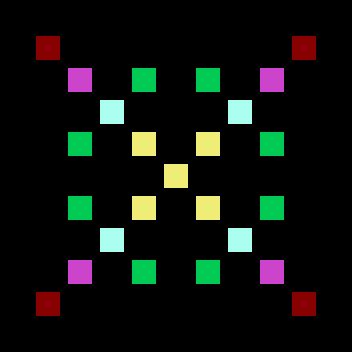
\includegraphics[width=1.3cm]{src/patterns/pixels/pixel_pattern6_14.png}%
} \\
        \midrule

        \makecell[l]{
\icode{.BYTE \$03,\$05,\$05,\$03,\$FD,\$FB,\$FB,\$FD}\\
\icode{.BYTE \$FB,\$FD,\$03,\$05,\$05,\$03,\$FD,\$FB}
} & \makecell[l]{

\includegraphics[width=1.3cm]{src/patterns/pixels/pixel_pattern6_15.png}%
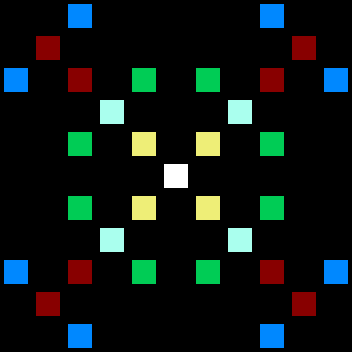
\includegraphics[width=1.3cm]{src/patterns/pixels/pixel_pattern6_16.png}%
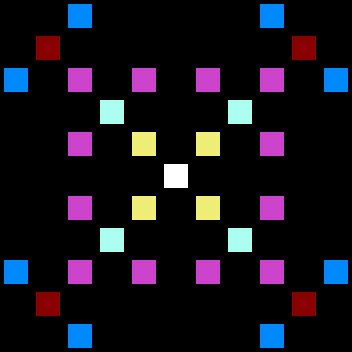
\includegraphics[width=1.3cm]{src/patterns/pixels/pixel_pattern6_17.png}%
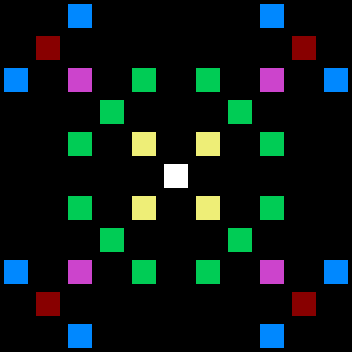
\includegraphics[width=1.3cm]{src/patterns/pixels/pixel_pattern6_18.png}%
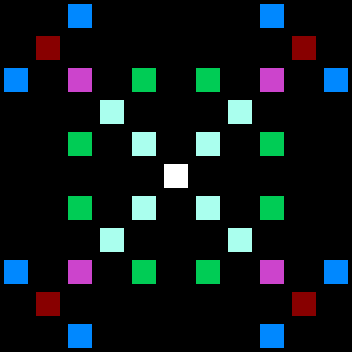
\includegraphics[width=1.3cm]{src/patterns/pixels/pixel_pattern6_19.png}%
} \\
        \midrule

        \makecell[l]{
\icode{.BYTE \$00}\\
\icode{.BYTE \$00}
} & \makecell[l]{
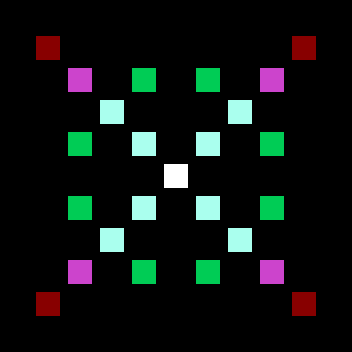
\includegraphics[width=1.3cm]{src/patterns/pixels/pixel_pattern6_20.png}%

\includegraphics[width=1.3cm]{src/patterns/pixels/pixel_pattern6_21.png}%
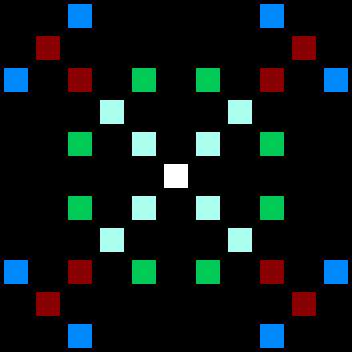
\includegraphics[width=1.3cm]{src/patterns/pixels/pixel_pattern6_22.png}%
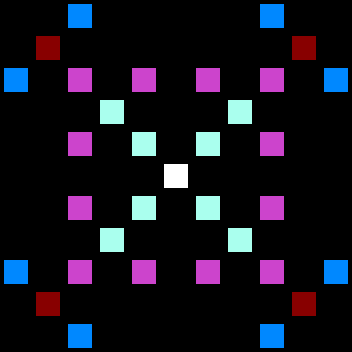
\includegraphics[width=1.3cm]{src/patterns/pixels/pixel_pattern6_23.png}%
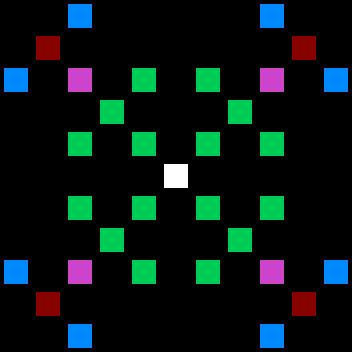
\includegraphics[width=1.3cm]{src/patterns/pixels/pixel_pattern6_24.png}%
} \\
        \midrule

          \end{tabular}
        \end{adjustbox}
      }\caption{Pattern Progression for 'Multi-Cross'}
    \end{figure}
    